\documentclass{article}
\usepackage{amsmath}
\usepackage{siunitx}
\usepackage{tikz}
\usepackage{graphicx}
\usepackage{mathpazo}
\usepackage[normalem]{ulem}
\usetikzlibrary{shapes, arrows}
\usepackage{hyperref}
\hypersetup{
    colorlinks=true,
    linkcolor=blue,
    filecolor=magenta,      
    urlcolor=cyan,
}
\usepackage[a4paper, margin=1.9cm]{geometry}
\usepackage{xepersian}


\title{موارد کاربردی سامانه}
\settextfont{XBZar}

\begin{document}
\maketitle
\section{معرفی کنشگرها}
\begin{itemize}
\item مشتری: مشتریها قابلیت ورود به سامانه و ایجاد حساب کاربری، ورود و ویرایش اطلاعات و ثبت درخواستهای تعریف شده توسط سیستم را دارند
\item کارمند: کارمندان وظیفه بررسی و تایید(رد) درخواستهای مشتریان و انجام آنها(در صورت تایید) و همچنین اطلاع موارد غیرعادی به مدیر را دارند.
\item مدیر: مدیر توانایی نظارت بر عملکرد مشتریها و کارمندان، لغو دسترسی آنها، ایجاد تراکنشهای جدید، تغییر قوانین، نظارت مالی بر سامانه و ایجاد کارمند و تعیین حقوق آنها را دارد
\end{itemize}
\section{نمودار موارد کاربرد}
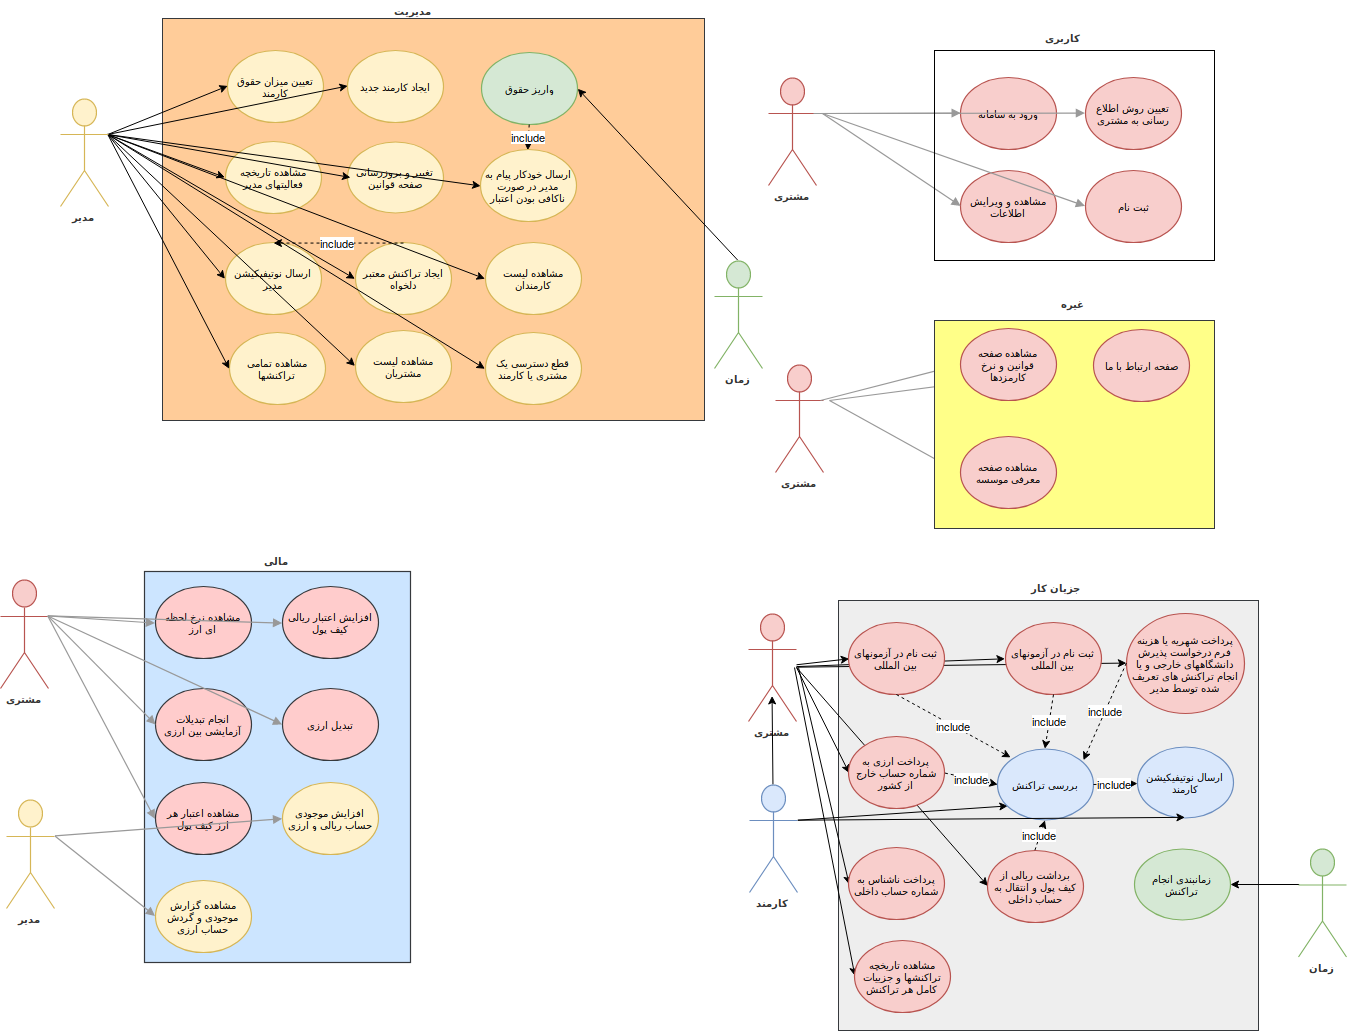
\includegraphics[width=17cm]{./Diagrams/all.png}
\newpage
\subsection{روابط بین کنشگرها}
\begin{center}

\includegraphics[scale=0.5]{./Diagrams/actors.png}
\end{center}
\section{توضیحات موارد کاربرد}
\begin{itemize}
\item \textbf{مورد کاربرد:}\\
مشاهده ی صفحه معرفی موسسه
\item \textbf{شناسه:}\\
1
\item \textbf{توضیح اجمالی:}\\
صفحه معرفی موسسه به کاربر نمایش داده میشود. 
\item \textbf{کنشگر اصلی:}\\
مشتری
\item \textbf{کنشگر فرعی:}\\
ندارد
\item \textbf{شرایط اولیه:}\\
ندارد
\item \textbf{روند اصلی:}\\
\begin{enumerate}
\item  این مورد کاربرد با درخواست کاربر برای مشاهدهی صفحه معرفی موسسه به کاربر شروع میشود
\item سامانه صفحه معرفی موسسه را به کاربر نمایش میدهد
\end{enumerate}
\item \textbf{شرایط پایانی:}\\ 
ندارد
\item \textbf{روندهای جایگزین:}\\
ندارد
\end{itemize}
\noindent\makebox[\linewidth]{\rule{\paperwidth}{0.4pt}}

\begin{itemize}
\item \textbf{مورد کاربرد:}\\
مشاهده نرخ لحظه ای ارز 
\item \textbf{شناسه:}\\
2
\item \textbf{توضیح اجمالی:}\\

در صفحه اولیه (خانه) کاربر نرخ لحظه ای ارزها را مشاهده میکند. 
\item \textbf{کنشگر اصلی:}\\
مشتری
\item \textbf{کنشگر فرعی:}\\
ندارد
\item \textbf{شرایط اولیه:}\\
ندارد
\item \textbf{روند اصلی:}\\
\begin{enumerate}
\item این مورد کاربرد با ورود کاربر به صفحه خانه شروع میشود
\item سامانه نرخ لحظه ای ارزها (دلار و یورو) را بر حسب ریال نشان میدهد. 
\end{enumerate}
\item \textbf{شرایط پایانی:}\\ 
ندارد
\item \textbf{روندهای جایگزین:}\\
ندارد
\end{itemize}
\noindent\makebox[\linewidth]{\rule{\paperwidth}{0.4pt}}
\begin{itemize}
\item \textbf{مورد کاربرد:}\\
مشاهده صفحه قوانین و نرخ کارمزدها 
\item \textbf{شناسه:}\\
۳
\item \textbf{توضیح اجمالی:}\\
صفحه قوانین و نرخ کارمزدها به کاربر نشان داده میشود. 
\item \textbf{کنشگر اصلی:}\\
مشتری
\item \textbf{کنشگر فرعی:}\\
ندارد
\item \textbf{شرایط اولیه:}\\
ندارد
\item \textbf{روند اصلی:}\\
\begin{enumerate}
\item  این مورد کاربرد با درخواست کاربر برای مشاهده صفحه قوانین و نرخ کارمزدها به کاربر شروع میشود.
\item سامانه قوانین و نرخ کارمزدها را به کاربر نشان میدهد.
\end{enumerate}
\item \textbf{شرایط پایانی:}\\ 
ندارد
\item \textbf{روندهای جایگزین:}\\
ندارد
\end{itemize}
\noindent\makebox[\linewidth]{\rule{\paperwidth}{0.4pt}}
\begin{itemize}
\item \textbf{مورد کاربرد:}\\
انجام تبدیلات آزمایشی بین ارزی 
\item \textbf{شناسه:}\\
4
\item \textbf{توضیح اجمالی:}\\
در صفحه اولیه (خانه) کاربر میتواند نتیجه تبدیل ارزها را با توجه به نرخ ارز و کارمزد به طور آزمایشی را مشاهده میکند. 
\item \textbf{کنشگر اصلی:}\\
مشتری
\item \textbf{کنشگر فرعی:}\\
ندارد
\item \textbf{شرایط اولیه:}\\
ندارد
\item \textbf{روند اصلی:}\\
\begin{enumerate}
\item این مورد کاربرد با ورود کاربر به صفحه خانه شروع میشود.
\item مشتری ارز مبدا، مقصد و مقدار دلخواه برای تبدیل را وارد میکند
\item در صورتی که مقدار ورودی صحیح باشد:
\begin{enumerate}
\item سامانه با توجه به نرخ لحظه ای ارز و مقدار کارمزد مقدار تبدیل شده صحیح را با توجه به ارز مقصد به مشتری نشان میدهد.  
\end{enumerate}
\item در غیر اینصورت:
\begin{enumerate}
\item سامانه پیغام خطایی مبنی بر نادرست بودن مقدار ورودی به مشتری میدهد
\end{enumerate}
\end{enumerate}
\item \textbf{شرایط پایانی:}\\ 
ندارد
\item \textbf{روندهای جایگزین:}\\
ندارد
\end{itemize}

\noindent\makebox[\linewidth]{\rule{\paperwidth}{0.4pt}}
\begin{itemize}
\item \textbf{مورد کاربرد:}\\
تغییر و بروزرسانی صفحه قوانین
\item \textbf{شناسه:}\\
5
\item \textbf{توضیح اجمالی:}\\
صفحه قوانین بروز میشود.
\item \textbf{کنشگر اصلی:}\\
مدیر
\item \textbf{کنشگر فرعی:}\\
ندارد
\item \textbf{شرایط اولیه:}\\
مدیر وارد داشبورد ادمین شده باشد.
\item \textbf{روند اصلی:}\\
\begin{enumerate}
\item  این مورد کاربرد با درخواست مدیر برای ایجاد تغییر در صفحه قوانین شروع میشود.
\item سامانه صفحه  ایجاد تغییر قوانین را به مدیر نشان میدهد.
\item مدیر کف و سقف مبلغ تراکنشها و توضیحات مربوط به قوانین سایت را تغییر میدهد.
\item پیغام بروزرسانی موفق قوانین به مدیر نشان داده میشود.
\end{enumerate}
\item \textbf{شرایط پایانی:}\\ 
قوانین یا سقف و کف مبلغ تراکنشها تغییر میکند و صفحه قوانین بروز میشود.
\item \textbf{روندهای جایگزین:}\\
ندارد
\end{itemize}

\noindent\makebox[\linewidth]{\rule{\paperwidth}{0.4pt}}

\begin{itemize}
\item \textbf{مورد کاربرد:}\\
ارسال نوتفیکیشن مدیر
\item \textbf{شناسه:}\\
6
\item \textbf{توضیح اجمالی:}\\
برای اطلاع رسانی مشتری ها از امکانات جدید نوتیفیکیشن با استفاده از رایانامه یا پیامک ارسال میشود.
\item \textbf{کنشگر اصلی:}\\
مدیر
\item \textbf{کنشگر فرعی:}\\
ندارد
\item \textbf{شرایط اولیه:}\\
مدیر وارد داشبورد مدیر شده باشد.
\item \textbf{روند اصلی:}\\
\begin{enumerate}
\item مورد کاربردی با درخواست مدیر در «ایجاد تراکنش معتبر دلخواه» شروع میشود: 
\item پیغام نوتیفیکیشن توسط مدیر پر میشود.
\item تمام مشتری ها به عنوان مشتری مقصد انتخاب میشوند.
\item با توجه به شیوه اطلاع رسانی ثبت شده توسط هر کدام از مشتری های مقصد پیغام مربوطه به آنها ارسال میشود.
\end{enumerate}

\item \textbf{شرایط پایانی:}\\ 
هر کدام از مشتریهای مقصد پیغام را از طریق روش اطلاع رسانی مشخص شده دریافت کند.
\item \textbf{روندهای جایگزین:}\\
ندارد
\end{itemize}
\noindent\makebox[\linewidth]{\rule{\paperwidth}{0.4pt}}

\begin{itemize}
\item \textbf{مورد کاربرد:}\\
ارسال نوتفیکیشن کارمند
\item \textbf{شناسه:}\\
7
\item \textbf{توضیح اجمالی:}\\
برای اطلاع رسانی مشتری ها از وضعیت درخواستشان نوتیفیکیشن با استفاده از رایانامه یا پیامک ارسال میشود.
\item \textbf{کنشگر اصلی:}\\
کارمند
\item \textbf{کنشگر فرعی:}\\
ندارد
\item \textbf{شرایط اولیه:}\\
کارمند وارد داشبورد کارمند شده باشد.
\item \textbf{روند اصلی:}\\
\begin{enumerate}
\item مورد کاربردی با درخواست کارمند در «بررسی تراکنش» شروع میشود
\item پیغام نوتیفیکیشن توسط کارمند وارد میشود.
\item مشتری مقصد برابر با مشتری در مورد کاربردی «بررسی تراکنش» یا «تایید تراکنش» میشود.
\item با توجه به شیوه اطلاع رسانی ثبت شده توسط مشتری مقصد پیغام مربوطه ارسال میشود.
\end{enumerate}

\item \textbf{شرایط پایانی:}\\ 
مشتری مقصد پیغام را از طریق روش اطلاع رسانی مشخص شده دریافت کند.
\item \textbf{روندهای جایگزین:}\\
ندارد
\end{itemize}
\noindent\makebox[\linewidth]{\rule{\paperwidth}{0.4pt}}

\begin{itemize}
\item \textbf{مورد کاربرد:}\\
ایجاد تراکنش معتبر دلخواه
\item \textbf{شناسه:}\\
8
\item \textbf{توضیح اجمالی:}\\
یک تراکنش دلخواه توسط مدیر تعریف میشود.
\item \textbf{کنشگر اصلی:}\\
مدیر
\item \textbf{کنشگر فرعی:}\\
ندارد
\item \textbf{شرایط اولیه:}\\
مدیر وارد داشبورد ادمین شده باشد.
\item \textbf{روند اصلی:}\\
\begin{enumerate}
\item  این مورد کاربرد با درخواست مدیر برای ایجاد یک تراکنش جدید شروع میشود.
\item سامانه صفحه ایجاد تراکنش جدید را به مدیر نشان میدهد.
\item مدیر عنوان تراکنش، مقدار هزینه آن، واحد پولی و کارمزد تراکنش و اطلاعات موردنیاز را وارد میکند.
\item در صورتی که این تراکنش از قبل در سامانه باشد:
\begin{enumerate}
\item سامانه پیغام خطا میدهد و به قسمت ۳ برمیگردد. 
\end{enumerate}

\item در غیراینصورت	:
\begin{enumerate}
\item پیغام ایجاد موفق تراکنش به مدیر نشان داده میشود.
\end{enumerate}
\item  درصورتی که مدیر گزینه ارسال نوتیفیکیشن را انتخاب کند:
\begin{enumerate}
\item مورد کابردی «ارسال نوتیفیکیشن مدیر» انجام میشود.
\end{enumerate}
\item سامانه پیغام ایجاد موفق تراکنش را نشان میدهد.
\end{enumerate}

\item \textbf{شرایط پایانی:}\\ 
در قسمت تراکنشهای مربوط به کاربران، تراکنش ایجاد شده اضافه شود.
\item \textbf{روندهای جایگزین:}\\
ندارد
\end{itemize}


\noindent\makebox[\linewidth]{\rule{\paperwidth}{0.4pt}}

\begin{itemize}
\item \textbf{مورد کاربرد:}\\
ثبت نام در آزمون های بین المللی
\item \textbf{شناسه:}\\
9
\item \textbf{توضیح اجمالی:}\\
درخواست مشتری برای ثبت نام در آزمون انتخابی، در سامانه ثبت میشود.
\item \textbf{کنشگر اصلی:}\\
مشتری
\item \textbf{کنشگر فرعی:}\\
ندارد
\item \textbf{شرایط اولیه:}\\
مشتری وارد داشبورد شده باشد.
\item \textbf{روند اصلی:}\\
\begin{enumerate}
\item  این مورد کاربرد با درخواست مشتری برای ثبت درخواست جدید شروع میشود.
\item سامانه صفحه درخواست جدید را به مشتری نشان میدهد.
\item مشتری نوع آزمون مورد نظر را انتخاب میکند.
\item سامانه اطلاعات موردنیاز برای ثبت نام را به مشتری نمایش میدهد
\item مشتری اطلاعات موردنیاز را وارد میکند(یا به صورت متن یا به صورت فایل)
\item سامانه هزینه ثبت نام را به مشتری نمایش میدهد
\item مشتری درخواست خود را ثبت میکند
\item در صورتی که موجودی مشتری کمتر از هزینه ثبت نام باشد سامانه :
\begin{enumerate}
\item سامانه پیغام خطا میدهد و روند جایگزین ۱ انجام میشود. 
\end{enumerate}

\item در غیراینصورت	:
\begin{enumerate}
\item پیغام ثبت موفق تراکنش به مشتری نشان داده میشود.
\item آدرس مربوط به کارمند مسئول بررسی درخواست به مشتری نمایش داده میشود.
\item مورد کاربردی «بررسی تراکنش» اجرا میشود.
\end{enumerate}

\end{enumerate}

\item \textbf{شرایط پایانی:}\\ 
در قسمت تراکنشهای مربوط به کارمند مسئول، تراکنش ایجاد شده در حالت در انتظار تایید اضافه شود.
\item \textbf{روندهای جایگزین:}\\
روند ۱:\\
\begin{enumerate}
\item پیغام ورود به کیف پول نمایش داده میشود.
\item کاربر ورود به کیف پول را تایید میکند.
\item مورد کاربردی «افزایش اعتبار ریالی کیف پول» اجرا میشود.؟؟
\end{enumerate}

\end{itemize}


\noindent\makebox[\linewidth]{\rule{\paperwidth}{0.4pt}}

\begin{itemize}
\item \textbf{مورد کاربرد:}\\
پرداخت شهریه یا هزینه فرم درخواست پذیرش دانشگاههای خارجی و یا انجام تراکنش های تعریف شده توسط مدیر
\item \textbf{شناسه:}\\
10
\item \textbf{توضیح اجمالی:}\\
درخواست مشتری برای پراخت هزینه پذیرش دانشگاههای خارجی در سامانه ثبت میشود.
\item \textbf{کنشگر اصلی:}\\
مشتری
\item \textbf{کنشگر فرعی:}\\
ندارد
\item \textbf{شرایط اولیه:}\\
مشتری وارد داشبورد شده باشد.
\item \textbf{روند اصلی:}\\
\begin{enumerate}
\item  این مورد کاربرد با درخواست مشتری برای ثبت درخواست جدید شروع میشود.
\item سامانه صفحه درخواست جدید را به مشتری نشان میدهد.
\item سامانه اطلاعات موردنیاز برای ثبت درخواست را به مشتری نمایش میدهد
\item مشتری اطلاعات موردنیاز را وارد میکند(یا به صورت متن یا به صورت فایل)
\item سامانه هزینه ثبت نام را به مشتری نمایش میدهد
\item مشتری درخواست خود را ثبت میکند
\item در صورتی که موجودی مشتری کمتر از هزینه ثبت نام باشد سامانه :
\begin{enumerate}
\item سامانه پیغام خطا میدهد و روند جایگزین ۱ انجام میشود. 
\end{enumerate}

\item در غیراینصورت	:
\begin{enumerate}
\item پیغام ثبت موفق تراکنش به مشتری نشان داده میشود.
\item آدرس مربوط به کارمند مسئول بررسی درخواست به مشتری نمایش داده میشود.
\item مورد کاربردی «بررسی تراکنش» اجرا میشود.
\end{enumerate}

\end{enumerate}

\item \textbf{شرایط پایانی:}\\ 
در قسمت تراکنشهای مربوط به کارمند مسئول، تراکنش ایجاد شده در حالت در انتظار تایید اضافه شود.
\item \textbf{روندهای جایگزین:}\\
روند ۱:\\
\begin{enumerate}
\item پیغام ورود به کیف پول نمایش داده میشود.
\item کاربر ورود به کیف پول را تایید میکند.
\item مورد کاربردی «افزایش اعتبار ریالی پول » اجرا میشود.؟؟
\end{enumerate}

\end{itemize}


\noindent\makebox[\linewidth]{\rule{\paperwidth}{0.4pt}}

\begin{itemize}
\item \textbf{مورد کاربرد:}\\
بررسی تراکنش
\item \textbf{شناسه:}\\
11
\item \textbf{توضیح اجمالی:}\\
کارمند درخواستهای دریافتی از مشتری ها را بررسی میکند.
\item \textbf{کنشگر اصلی:}\\
کارمند
\item \textbf{کنشگر فرعی:}\\
ندارد
\item \textbf{شرایط اولیه:}\\
کارمند وارد داشبورد کارمند شده باشد.
\item \textbf{روند اصلی:}\\
\begin{enumerate}
\item  این مورد کاربرد با درخواست کارمند برای بررسی درخواست جدید شروع میشود.
\item سامانه صفحه بررسی درخواست جدید را به کارمند نشان میدهد.
\item کارمند یکی از درخواست ها را انتخاب میکند.
\item در صورتی که وضعیت درخواست درانتظار تایید نباشد:
\begin{enumerate}
\item در همان صفحه میماند و وارد وضعیت ۳ میشود.
\end{enumerate}
\item در غیر این صورت:
\begin{enumerate}
\item سامانه صفحه مربوط به اطلاعات درخواست مشتری را به کارمند نشان میدهد.
\item کارمند اطلاعات مشتری را بررسی میکند.
\item در صورت صحت اطلاعات:
\begin{enumerate}
\item کارمند وضعیت درخواست را به درحال رسیدگی تغییر میدهد.
\item هزینه تراکنش و کارمزد آن محاسبه میشود
\item هزینه محاسبه شده از حساب ریالی مشتری کم شده و به حساب ریالی شرکت اضافه میشود
\item کارمند ارسال نوتیفیکیشن را تایید میکند
\item مورد کاربردی  «ارسال نوتیفیکیشن کارمند» انجام میشود.
\end{enumerate}
\item در غیر اینصورت:
\begin{enumerate}
\item  در صورتی که کارمند مورد غیر عادی متوجه شود وضعیت تراکنش را غیرعادی میکند.
\item در غیر این صورت وضعیت تراکنش را لغوشده اعلام میکند.
\item کارمند ارسال نوتیفیکیشن را تایید میکند
\item مورد کاربردی  «ارسال نوتیفیکیشن کارمند» انجام میشود.
\end{enumerate}
\end{enumerate}

\end{enumerate}

\item \textbf{شرایط پایانی:}\\ 
در قسمت تراکنشهای مربوط به مشتری، تراکنش درخواستی در وضعیت تایید باشد.\\
مقدار هزینه انجام تراکنش از حساب مشتری کم شده و به حساب ریالی شرکت اضافه شده باشد.\\
\item \textbf{روندهای جایگزین:}\\


\end{itemize}

\noindent\makebox[\linewidth]{\rule{\paperwidth}{0.4pt}}

\begin{itemize}
\item \textbf{مورد کاربرد:}\\
زمانبندی انجام تراکنشها
\item \textbf{شناسه:}\\
12
\item \textbf{توضیح اجمالی:}\\
تمام درخواستها بررسی میشوند و هر درخواستی که از مهلت آن بیش از 24 ساعت گذشته باشد لغو میشود.
\item \textbf{کنشگر اصلی:}\\
زمان
\item \textbf{کنشگر فرعی:}\\
کارمند
\item \textbf{شرایط اولیه:}\\
ندارد
\item \textbf{روند اصلی:}\\
\begin{enumerate}
\item در دوره های زمانی منظم اجرا میشود.
\item سامانه تمام درخواست های ثبت شده را مشاهده میکند
\item هر درخواستی که از زمان شروع آن بیش از 24 ساعت گذشته باشد و جزو درخواستهای تایید نشده باشد به وضعیت لغو در می آید
\item  با توجه به شیوه اطلاع رسانی ثبت شده توسط مشتریهای مربوط به درخواستهای لغو شده پیغام لغو تراکنش برای آنها ارسال میشود.

\end{enumerate}

\item \textbf{شرایط پایانی:}\\ 
وضعیت درخواستهای مشتریانی(و نیز درخواستهای مربوطه در قسمت کارمندان) که بیش از 24 ساعت از آن گذشته و تایید نشده اند به حالت لغو در می آید.\\
\item \textbf{روندهای جایگزین:}\\

\end{itemize}

\noindent\makebox[\linewidth]{\rule{\paperwidth}{0.4pt}}

\begin{itemize}
\item \textbf{مورد کاربرد:}\\
ثبت نام
\item \textbf{شناسه:}\\
13
\item \textbf{توضیح اجمالی:}\\
کاربر در سایت ثبت نام میکند.
\item \textbf{کنشگر اصلی:}\\
مشتری
\item \textbf{کنشگر فرعی:}\\
ندارد
\item \textbf{شرایط اولیه:}\\
ندارد
\item \textbf{روند اصلی:}\\
\begin{enumerate}
\item  این مورد کاربرد با درخواست کاربر برای مشاهده ی صفحه ثبت نام به کاربر شروع میشود
\item سامانه صفحه ثبت نام را به کاربر نمایش میدهد
\item کاربر قسمتهای نام و نام خانوادگی، نام کاربری، شماره تماس، ایمیل، رمز عبور و تکرار رمز عبور را پر میکند.
\item کاربر گزینه ثبت نام را انتخاب میکند
\item در صورتی که هر کدام از قسمتهای ذکر شده در ۳ خالی بماند، سیستم پیام «اطلاعات ناقص» را نمایش میدهد و به ۳ میرود.
\item  در صورتی که ایمیل فرمت اشتباه داشته باشد سیستم پیام «ایمیل اشتباه» میدهد و به ۳ برمیگردد
\item در صورتی که رمز عبور و تکرار رمز عبور یکی نباشند سیستم پیام «عدم تطابق رمز عبور» میدهد و به ۳ برمیگردد.
\item در صورتی که نام کاربری وارد شده از قبل در سامانه وجود داشته باشد، سیستم پیام «نام کاربری تکراری» میدهد و به ۳ برمیگردد
\item در صورتی که ایمیل وارد شده از قبل در سامانه وجود داشته باشد، سیستم پیام «ایمیل تکراری» میدهد و به ۳ برمیگردد.
\item در صورتی که موارد 5 تا9 رخ ندهد سیستم پیام «ثبت نام موفق» را به کاربر نمایش میدهد.
\end{enumerate}
\item \textbf{شرایط پایانی:}\\ 
اطلاعات کاربر در (دیتابیس) سامانه به عنوان کاربر ذخیره شده و یک شماره حساب به کاربر اختصاص داده شود.
\item \textbf{روندهای جایگزین:}\\
ندارد
\end{itemize}
\noindent\makebox[\linewidth]{\rule{\paperwidth}{0.4pt}}

\begin{itemize}
\item \textbf{مورد کاربرد:}\\
مشاهده و ویرایش اطلاعات
\item \textbf{شناسه:}\\
14
\item \textbf{توضیح اجمالی:}\\
کاربر اطلاعات خود را مشاهده کرده و میتواند اطلاعات خود را ویرایش کند.
\item \textbf{کنشگر اصلی:}\\
مشتری
\item \textbf{کنشگر فرعی:}\\
ندارد
\item \textbf{شرایط اولیه:}\\
کاربر وارد داشبورد شده باشد.
\item \textbf{روند اصلی:}\\
\begin{enumerate}
\item  این مورد کاربرد با درخواست کاربر برای مشاهده اطلاعات در داشبورد شروع میشود
\item سامانه صفحه  اطلاعات را به کاربر نمایش میدهد
\item در صورتی که کاربر گزینه ویرایش اطلاعات را انتخاب کند:
\begin{enumerate}
\item صفحه ویرایش اطلاعات به کاربر نشان داده میشود.
\item کاربر قسمت های نام یا نام خانوادگی یا شماره تماس یا ایمیل و یا رمز عبور و تکرار رمز عبور را تغییر میدهد.
\item  در صورتی که ایمیل فرمت اشتباه داشته باشد سیستم پیام «ایمیل اشتباه» میدهد و به ۳.ب برمیگردد
\item در صورتی که رمز عبور و تکرار رمز عبور یکی نباشند سیستم پیام «عدم تطابق رمز عبور» میدهد و به ۳.ب برمیگردد.
\item در صورتی که ایمیل وارد شده از قبل در سامانه وجود داشته باشد، سیستم پیام «ایمیل تکراری» میدهد و به ۳.ب برمیگردد.
\item در صورتی که موارد ۳.ج تا ۳.ه رخ ندهد سیستم پیام «تغییر اطلاعات موفق» را به کاربر نمایش میدهد.
\end{enumerate}
\end{enumerate}
\item \textbf{شرایط پایانی:}\\ 
در صورتی که کاربر اطلاعات خود را تغییر دهد، اطلاعات جدید کاربر در (دیتابیس) سامانه به عنوان کاربر ذخیره شده باشد.
\item \textbf{روندهای جایگزین:}\\
ندارد
\end{itemize}
\noindent\makebox[\linewidth]{\rule{\paperwidth}{0.4pt}}

\begin{itemize}
\item \textbf{مورد کاربرد:}\\
مشاهده اعتبار هر ارز کیف پول
\item \textbf{شناسه:}\\
15
\item \textbf{توضیح اجمالی:}\\
کاربر مقدار اعتبار هر ارز مربوط به کیف پول خود را مشاهده میکند.
\item \textbf{کنشگر اصلی:}\\
مشتری
\item \textbf{کنشگر فرعی:}\\
ندارد
\item \textbf{شرایط اولیه:}\\
کاربر وارد داشبورد  شده باشد.
\item \textbf{روند اصلی:}\\
\begin{enumerate}
\item  این مورد کاربرد با درخواست کاربر برای مشاهده کیف پول در داشبورد شروع میشود
\item سامانه صفحه  مربوط به کیف پول را به کاربر نمایش میدهد
\item کاربر میتواند اعتبار هر کدام از ارزهای مربوط به کیف پول خود را مشاهده کند.

\end{enumerate}
\item \textbf{شرایط پایانی:}\\ 
\item \textbf{روندهای جایگزین:}\\
ندارد
\end{itemize}
\noindent\makebox[\linewidth]{\rule{\paperwidth}{0.4pt}}


\begin{itemize}
\item \textbf{مورد کاربرد:}\\
افزایش اعتبار ریالی کیف پول
\item \textbf{شناسه:}\\
16
\item \textbf{توضیح اجمالی:}\\
کاربر اعتبار ریالی کیف پول خود را افزایش میدهد.
\item \textbf{کنشگر اصلی:}\\
مشتری
\item \textbf{کنشگر فرعی:}\\
ندارد
\item \textbf{شرایط اولیه:}\\
کاربر وارد داشبورد شده باشد.
\item \textbf{روند اصلی:}\\
\begin{enumerate}
\item  این مورد کاربرد با درخواست کاربر برای مشاهده کیف پول در داشبورد شروع میشود
\item سامانه صفحه  کیف پول را به کاربر نمایش میدهد
\item کاربر گزینه افزایش اعتبار ریالی کیف پول را انتخاب میکند.
\item کاربر مبلغ مورد نظر را بر حسب ریال وارد میکند.
\item کاربر تایید را انتخاب میکند.
\item سیستم پیام «افزایش اعتبار ریالی موفق» را به کاربر نمایش میدهد.
\end{enumerate}
\item \textbf{شرایط پایانی:}\\ 
در (دیتابیس) سامانه مقدار اعتبار ریالی مربوط به کاربر طبق مقدار اضافه شده افزایش یابد.
\item \textbf{روندهای جایگزین:}\\
ندارد
\end{itemize}
\noindent\makebox[\linewidth]{\rule{\paperwidth}{0.4pt}}


\begin{itemize}
\item \textbf{مورد کاربرد:}\\
تبدیل ارزی
\item \textbf{شناسه:}\\
17
\item \textbf{توضیح اجمالی:}\\
کاربر میتواند مقداری از موجودی ارزی خود را به ارز دیگری تبدیل کند.
\item \textbf{کنشگر اصلی:}\\
مشتری
\item \textbf{کنشگر فرعی:}\\
ندارد
\item \textbf{شرایط اولیه:}\\
کاربر وارد داشبورد مشتری شده باشد.
\item \textbf{روند اصلی:}\\
\begin{enumerate}
\item  این مورد کاربرد با درخواست کاربر برای مشاهده کیف پول در داشبورد شروع میشود
\item سامانه صفحه  کیف پول را به کاربر نمایش میدهد
\item کاربر گزینه  تبدیل ارزی را انتخاب میکند
\item  کاربر ارز مبدا، مقصد و مقدار دلخواه برای تبدیل را وارد میکند و تایید میکند.
\item در صورتی که مقدار ورودی صحیح باشد:
\begin{enumerate}
\item سامانه با توجه به نرخ لحظه ای ارز و مقدار کارمزد مقدار تبدیل شده صحیح را با توجه به ارز مقصد به مشتری نشان میدهد.  
\item در صورتی که کاربر تایید کند:
\item مقدار مورد نظر از حساب ارزی مبدا برداشت و به حساب ارزی مقصد واریز میشود.
\end{enumerate}
\item در غیر اینصورت:
\begin{enumerate}
\item  سامانه پیغام خطایی مبنی بر نادرست بودن مقدار ورودی به مشتری میدهد و به قسمت ۴ برمیگردد.
\end{enumerate}
\end{enumerate}
\item \textbf{شرایط پایانی:}\\ 
در (دیتابیس) سامانه از مقدار ارزی مبدا مربوط به کاربر کاسته و به مقدار ارزی مقصد مربوط به کاربر اضافه شده باشد.
\item \textbf{روندهای جایگزین:}\\
ندارد
\end{itemize}
\noindent\makebox[\linewidth]{\rule{\paperwidth}{0.4pt}}

\begin{itemize}
\item \textbf{مورد کاربرد:}\\
مشاهده تاریخچه تراکنش ها و جزییات کامل هر تراکنش
\item \textbf{شناسه:}\\
18
\item \textbf{توضیح اجمالی:}\\
کاربر تاریخچه تراکنشها و جزییات هر کدام از آنها را مشاهده کند.
\item \textbf{کنشگر اصلی:}\\
مشتری
\item \textbf{کنشگر فرعی:}\\
ندارد
\item \textbf{شرایط اولیه:}\\
کاربر وارد داشبورد مشتری شده باشد.
\item \textbf{روند اصلی:}\\
\begin{enumerate}
\item  این مورد کاربرد با درخواست کاربر برای مشاهده تاریخچه تراکنشها در داشبورد شروع میشود
\item سامانه صفحه  تاریخچه تراکنشها را به کاربر نمایش میدهد
\item کاربر لاگ مربوط به تراکنشها را مشاهده میکند.
\item  در صورتی که کاربر قسمت جزییات مربوط به هرکدام از تراکنشها را انتخاب کند
\item سامانه صفحه جزییات مربوط به تراکنش انتخابی شامل وضعیت بررسی تراکنش، کارمند مربوط به تراکنش، نام و مقدار هزینه تراکنش، اطلاعات اضافی، فایلهای آپلود شده و نظر کارمند موردنظر را نمایش میدهد.
\end{enumerate}
\item \textbf{شرایط پایانی:}\\ 
ندارد
\item \textbf{روندهای جایگزین:}\\
ندارد
\end{itemize}
\noindent\makebox[\linewidth]{\rule{\paperwidth}{0.4pt}}

\begin{itemize}
\item \textbf{مورد کاربرد:}\\
تعیین روش اطلاع رسانی به مشتری
\item \textbf{شناسه:}\\
19
\item \textbf{توضیح اجمالی:}\\
کاربر نحوه اطلاع رسانی بخود را مشخص میکند
\item \textbf{کنشگر اصلی:}\\
مشتری
\item \textbf{کنشگر فرعی:}\\
ندارد
\item \textbf{شرایط اولیه:}\\
کاربر وارد داشبورد مشتری شده باشد.
\item \textbf{روند اصلی:}\\
\begin{enumerate}
\item  این مورد کاربرد با درخواست کاربر برای تعیین روش اطلاع رسانی در داشبورد شروع میشود
\item سامانه صفحه انتخاب روش اطلاع رسانی را به کاربر نمایش میدهد
\item کاربر یکی از دو گزینه اطلاع رسانی با پیامک و اطلاع رسانی با ایمیل را انتخاب میکند.
\item  سامانه پیغام «انتخاب روش اطلاع رسانی موفق» را نمایش میدهد.
\end{enumerate}
\item \textbf{شرایط پایانی:}\\ 
در (دیتابیس) سامانه روش اطلاع رسانی مربوط به کاربر با توجه به روش انتخابی اش ذخیره شود.
\item \textbf{روندهای جایگزین:}\\
ندارد
\end{itemize}
\noindent\makebox[\linewidth]{\rule{\paperwidth}{0.4pt}}


\begin{itemize}
\item \textbf{مورد کاربرد:}\\
مشاهده تمامی تراکنشها
\item \textbf{شناسه:}\\
20
\item \textbf{توضیح اجمالی:}\\
مدیر میتواند تمامی تراکنشها را مشاهده میکند.
\item \textbf{کنشگر اصلی:}\\
مدیر
\item \textbf{کنشگر فرعی:}\\
ندارد
\item \textbf{شرایط اولیه:}\\
کاربر وارد داشبورد مدیر(ادمین) شده باشد.
\item \textbf{روند اصلی:}\\
\begin{enumerate}
\item  این مورد کاربرد با درخواست کاربر برای مشاهده تمامی تراکنشها در داشبورد شروع میشود
\item سامانه صفحه مربوط به تمامی تراکنشها را به کاربر نمایش میدهد
\item کاربر لاگ مربوط به تراکنشها را مشاهده میکند.
\item  در صورتی که کاربر قسمت جزییات مربوط به هرکدام از تراکنشها را انتخاب کند
\item سامانه صفحه جزییات مربوط به تراکنش انتخابی شامل وضعیت بررسی تراکنش، مشتری مربوط به تراکنش، کارمند مربوط به تراکنش، نام و مقدار هزینه تراکنش، اطلاعات اضافی، فایلهای آپلود شده و نظر کارمند موردنظر را نمایش میدهد.
\end{enumerate}
\item \textbf{شرایط پایانی:}\\ 
ندارد.
\item \textbf{روندهای جایگزین:}\\
ندارد
\end{itemize}
\noindent\makebox[\linewidth]{\rule{\paperwidth}{0.4pt}}

\begin{itemize}
\item \textbf{مورد کاربرد:}\\
مشاهده لیست مشتریان
\item \textbf{شناسه:}\\
21
\item \textbf{توضیح اجمالی:}\\
مدیر میتواند تمامی مشتریها را مشاهده میکند.
\item \textbf{کنشگر اصلی:}\\
مدیر
\item \textbf{کنشگر فرعی:}\\
ندارد
\item \textbf{شرایط اولیه:}\\
کاربر وارد داشبورد مدیر(ادمین) شده باشد.
\item \textbf{روند اصلی:}\\
\begin{enumerate}
\item  این مورد کاربرد با درخواست کاربر برای مشاهده تمامی  مشتریها در داشبورد شروع میشود
\item سامانه صفحه مربوط به تمامی مشتریها را به کاربر نمایش میدهد
\item کاربر نام هر یک از مشتریها را مشاهده میکند.
\item  در صورتی که کاربر قسمت جزییات مربوط به هرکدام از مشتریها را انتخاب کند
\item سامانه صفحه جزییات مربوط به مشتری انتخابی شامل اطلاعات پروفایل مشتری(نام و نام خانوادگی، نام کاربری، ایمیل، شماره تلفن) و اطلاعات کیف پول(مقدار پول در هر کدام یک از ارزها) را نمایش میدهد.
\end{enumerate}
\item \textbf{شرایط پایانی:}\\ 
ندارد.
\item \textbf{روندهای جایگزین:}\\
ندارد
\end{itemize}
\noindent\makebox[\linewidth]{\rule{\paperwidth}{0.4pt}}

\begin{itemize}
\item \textbf{مورد کاربرد:}\\
مشاهده لیست کارمندان
\item \textbf{شناسه:}\\
22
\item \textbf{توضیح اجمالی:}\\
مدیر میتواند تمامی کارمندان را مشاهده میکند.
\item \textbf{کنشگر اصلی:}\\
مدیر
\item \textbf{کنشگر فرعی:}\\
ندارد
\item \textbf{شرایط اولیه:}\\
کاربر وارد داشبورد مدیر(ادمین) شده باشد.
\item \textbf{روند اصلی:}\\
\begin{enumerate}
\item  این مورد کاربرد با درخواست کاربر برای مشاهده تمامی  کارمندان در داشبورد شروع میشود
\item سامانه صفحه مربوط به تمامی کارمندان را به کاربر نمایش میدهد
\item کاربر نام هر یک از کارمندان را مشاهده میکند.
\item  در صورتی که کاربر قسمت جزییات مربوط به هرکدام از کارمندان را انتخاب کند
\item سامانه صفحه جزییات مربوط به کارمند انتخابی شامل اطلاعات پروفایل کارمند(نام و نام خانوادگی، نام کاربری، ایمیل، شماره تلفن) و اطلاعات کیف پول(مقدار پول در هر کدام یک از ارزها) و مقدار حقوق دریافتی کارمند را نمایش میدهد.
\end{enumerate}
\item \textbf{شرایط پایانی:}\\ 
ندارد.
\item \textbf{روندهای جایگزین:}\\
ندارد
\end{itemize}
\noindent\makebox[\linewidth]{\rule{\paperwidth}{0.4pt}}

\begin{itemize}
\item \textbf{مورد کاربرد:}\\
قطع دسترسی یک مشتری یا کارمند
\item \textbf{شناسه:}\\
23
\item \textbf{توضیح اجمالی:}\\
مدیر میتواند دسترسی یک مشتری یا کارمند را از سامانه قطع کند.
\item \textbf{کنشگر اصلی:}\\
مدیر
\item \textbf{کنشگر فرعی:}\\
ندارد
\item \textbf{شرایط اولیه:}\\
کاربر وارد داشبورد مدیر(ادمین) شده باشد.
\item \textbf{روند اصلی:}\\
\begin{enumerate}
\item  این مورد کاربرد با درخواست کاربر برای مشاهده تمامی کارمندان یا مشتریان در داشبورد شروع میشود
\item سامانه صفحه مربوط به تمامی کارمندان یا مشتریان را به کاربر نمایش میدهد
\item کاربر نام هر یک از کارمندان یا مشتریان را مشاهده میکند.
\item  در صورتی که کاربر قسمت قطع دسترسی مربوط به هرکدام از کارمندان یا مشتریان را انتخاب کند
\item پیغام «قطع دسترسی موفق» به کاربر نمایش داده میشود.
\end{enumerate}
\item \textbf{شرایط پایانی:}\\ 
در هنگام ورود کارمند یا مشتری ممنوع شده به سامانه، پیام «ورود ممنوع» به کاربر نشان داده میشود و کاربر نمیتواند وارد سامانه شود.
\item \textbf{روندهای جایگزین:}\\
ندارد
\end{itemize}
\noindent\makebox[\linewidth]{\rule{\paperwidth}{0.4pt}}


\begin{itemize}
\item \textbf{مورد کاربرد:}\\
ورود به سامانه
\item \textbf{شناسه:}\\
24
\item \textbf{توضیح اجمالی:}\\
کاربر وارد سامانه میشود.
\item \textbf{کنشگر اصلی:}\\
مشتری
\item \textbf{کنشگر فرعی:}\\
ندارد
\item \textbf{شرایط اولیه:}\\
ندارد
\item \textbf{روند اصلی:}\\
\begin{enumerate}
\item  این مورد کاربرد با درخواست کاربر برای ورود به سامانه شروع میشود
\item سامانه صفحه ورود را به کاربر نمایش میدهد
\item کاربر قسمتهای نام کاربری و رمز عبور را پر میکند.
\item کاربر گزینه ورود را انتخاب میکند
\item در صورتی که هر کدام از قسمتهای ذکر شده در ۳ خالی بماند، سیستم پیام «اطلاعات ناقص» را نمایش میدهد و به ۳ میرود.
\item  در صورتی که نام کاربری وجود نداشته باشد و یا رمز عبور اشتباه باشد، سیستم پیام «رمز عبور و یا نام کاربری اشتباه» میدهد و به ۳ برمیگردد
\item در غیر اینصورت سیستم پیام «ورود موفق» را به کاربر نشان میدهد.
\end{enumerate}
\item \textbf{شرایط پایانی:}\\ 
کاربر پس از ورود با توجه به نوعش (مشتری، کارمند و یا مدیر) میتواند وارد داشبورد خود شود. (داشبورد مربوطه به عنوان یک گزینه در صفحه اولیه وجود خواهد داشت)
\item \textbf{روندهای جایگزین:}\\
ندارد
\end{itemize}
\noindent\makebox[\linewidth]{\rule{\paperwidth}{0.4pt}}

\begin{itemize}
\item \textbf{مورد کاربرد:}\\
افزایش موجودی حساب ریالی و ارزی موسسه
\item \textbf{شناسه:}\\
25
\item \textbf{توضیح اجمالی:}\\
مدیر مقدار موجودی سامانه را افزایش میدهد.
\item \textbf{کنشگر اصلی:}\\
مدیر
\item \textbf{کنشگر فرعی:}\\
ندارد
\item \textbf{شرایط اولیه:}\\
مدیر وارد داشبورد شده باشد.
\item \textbf{روند اصلی:}\\
\begin{enumerate}
\item  این مورد کاربرد با درخواست کاربر برای ورود به افزایش موجودی شروع میشود
\item سامانه صفحه افزایش موجودی را به کاربر نمایش میدهد
\item کاربر نوع ارز مورد نظر و مقدار افزایش را وارد میکند.
\item کاربر افزایش را تایید میکند.
\item  سیستم پیام «افزایش موجودی موفق» را به کاربر نشان میدهد.
\end{enumerate}
\item \textbf{شرایط پایانی:}\\ 
مقدار موجودی سامانه، با توجه به نوع ارز و مقدار افزایش یافته در (دیتابیس) سامانه تغییر کند.
\item \textbf{روندهای جایگزین:}\\
ندارد
\end{itemize}
\noindent\makebox[\linewidth]{\rule{\paperwidth}{0.4pt}}



\begin{itemize}
\item \textbf{مورد کاربرد:}\\
ایجاد کارمند جدید
\item \textbf{شناسه:}\\
26
\item \textbf{توضیح اجمالی:}\\
مدیر یک کارمند جدید تعریف میکند.
\item \textbf{کنشگر اصلی:}\\
مدیر
\item \textbf{کنشگر فرعی:}\\
کارمند
\item \textbf{شرایط اولیه:}\\
کارمند به عنوان مشتری در سایت ثبت نام کرده باشد و مدیر وارد داشبورد شده باشد.
\item \textbf{روند اصلی:}\\
\begin{enumerate}
\item  این مورد کاربرد با درخواست مدیر برای ورود به قسمت مشتری ها شروع میشود
\item سامانه صفحه مشتریها را به مدیر نمایش میدهد
\item مدیر فرد مورد نظر را پیدا کرده و گزینه تبدیل به کارمند را انتخاب میکند..
\item  سیستم پیام «ایجاد کارمند موفق» را به کاربر نشان میدهد.
\end{enumerate}
\item \textbf{شرایط پایانی:}\\ 
مشتری که تبدیل به کارمند شده است بعد از ورود به سامانه میتواند وارد داشبورد کارمند شود.
\item \textbf{روندهای جایگزین:}\\
ندارد
\end{itemize}
\noindent\makebox[\linewidth]{\rule{\paperwidth}{0.4pt}}


\begin{itemize}
\item \textbf{مورد کاربرد:}\\
مشاهده گزارش موجودی و گردش حساب ارزی
\item \textbf{شناسه:}\\
27
\item \textbf{توضیح اجمالی:}\\
مدیر موجودی و گردش حساب را مشاهده میکند.
\item \textbf{کنشگر اصلی:}\\
مدیر
\item \textbf{کنشگر فرعی:}\\
ندارد
\item \textbf{شرایط اولیه:}\\
مدیر وارد داشبورد شده باشد.
\item \textbf{روند اصلی:}\\
\begin{enumerate}
\item  این مورد کاربرد با درخواست کاربر برای ورود به مشاهده گزارش موجودی و گردش حساب ارزی شروع میشود
\item سامانه صفحه مشاهده گزارش موجودی و گردش حساب ارزی را به کاربر نمایش میدهد
\item کاربر میتواند مقدار موجودی سامانه در هر کدام از ارزها و همچنین مقدار پرداختی ها را مشاهده کند.
\end{enumerate}
\item \textbf{شرایط پایانی:}\\ 
ندارد
\item \textbf{روندهای جایگزین:}\\
ندارد
\end{itemize}
\noindent\makebox[\linewidth]{\rule{\paperwidth}{0.4pt}}


\begin{itemize}
\item \textbf{مورد کاربرد:}\\
تعیین میزان حقوق هر کارمند
\item \textbf{شناسه:}\\
28
\item \textbf{توضیح اجمالی:}\\
مدیر مقدار حقوق هر کارمند را تعیین میکند.
\item \textbf{کنشگر اصلی:}\\
مدیر
\item \textbf{کنشگر فرعی:}\\
ندارد
\item \textbf{شرایط اولیه:}\\
مدیر وارد داشبورد شده باشد.
\item \textbf{روند اصلی:}\\
\begin{enumerate}
\item  این مورد کاربرد با درخواست کاربر برای مشاهده تمامی  کارمندان در داشبورد شروع میشود
\item سامانه صفحه مربوط به تمامی کارمندان را به کاربر نمایش میدهد
\item کاربر نام هر یک از کارمندان را مشاهده میکند.
\item  در صورتی که کاربر قسمت جزییات مربوط به هرکدام از کارمندان را انتخاب کند
\item سامانه صفحه جزییات مربوط به کارمند را به کاربر نشان میدهد
\item مدیر در قسمت حقوق مقدار حقوق دریافتی کارمند را تعیین میکند
\item مدیر مقدار مشخص شده را تایید میکند
\item سامانه پیام «تعیین حقوق موفق» را به کاربر نشان میدهد.
\end{enumerate}
\item \textbf{شرایط پایانی:}\\ 
مقدار حقوق کارمند در (دیتابیس) سامانه تغییر کند.
\item \textbf{روندهای جایگزین:}\\
ندارد
\end{itemize}
\noindent\makebox[\linewidth]{\rule{\paperwidth}{0.4pt}}

\begin{itemize}
\item \textbf{مورد کاربرد:}\\
ارسال خودکار پیام به مدیر در صورت ناکافی بودن اعتبار ریالی
\item \textbf{شناسه:}\\
29
\item \textbf{توضیح اجمالی:}\\
در صورتی که اعتبار ریالی سامانه کافی نباشد پیام هشدار به مدیر داده میشود.
\item \textbf{کنشگر اصلی:}\\
زمان
\item \textbf{کنشگر فرعی:}\\
مدیر
\item \textbf{شرایط اولیه:}\\
ندارد
\item \textbf{روند اصلی:}\\
\begin{enumerate}
\item  این مورد کاربرد بعد از مورد کاربردی «واریز حقوق» شروع میشود
\item پیام «موجودی ناکافی» در داشبورد مدیر نمایش داده میشود.
\end{enumerate}
\item \textbf{شرایط پایانی:}\\ 
ندارد
\item \textbf{روندهای جایگزین:}\\
ندارد
\end{itemize}
\noindent\makebox[\linewidth]{\rule{\paperwidth}{0.4pt}}


\begin{itemize}
\item \textbf{مورد کاربرد:}\\
واریز حقوق
\item \textbf{شناسه:}\\
30
\item \textbf{توضیح اجمالی:}\\
حقوق کارمندان از حساب ریالی سامانه پرداخت میشود.
\item \textbf{کنشگر اصلی:}\\
زمان
\item \textbf{کنشگر فرعی:}\\
ندارد
\item \textbf{شرایط اولیه:}\\
ندارد
\item \textbf{روند اصلی:}\\
\begin{enumerate}
\item  این مورد کاربردی در دوره های زمانی منظم اجرا میشود.
\item با توجه به میزان حقوق هر یک از کارمندان مقدار حقوق از حساب ریالی سامانه کم شده و به حساب ریالی کارمندان اضافه میشود.
\item در صورتی که میزان موجودی حساب ریالی کافی نباشد مورد کاربردی «ارسال خودکار پیام به مدیر در صورت ناکافی بودن اعتبار ریالی» اجرا میشود.
\end{enumerate}
\item \textbf{شرایط پایانی:}\\ 
مقدار موجودی حساب ریالی سامانه و هر یک از کارمندان به درستی به روز شود.
\item \textbf{روندهای جایگزین:}\\
ندارد
\end{itemize}
\noindent\makebox[\linewidth]{\rule{\paperwidth}{0.4pt}}


\begin{itemize}
\item \textbf{مورد کاربرد:}\\
صفحه ارتباط با ما
\item \textbf{شناسه:}\\
31
\item \textbf{توضیح اجمالی:}\\
کاربر می‌تواند صفحه ارتباط با ما را مشاهده کند و پیام خود را بفرستد.
\item \textbf{کنشگر اصلی:}\\
مشتری
\item \textbf{کنشگر فرعی:}\\
ندارد
\item \textbf{شرایط اولیه:}\\
ندارد
\item \textbf{روند اصلی:}\\
\begin{enumerate}
\item  این مورد کاربردی با درخواست کاربر برای مشاهده صفحه ارتباط با ما شروع میشود
\item سامانه صفحه ارتباط با ما را به کاربر نشان میدهد
\item کاربر قسمت ایمیل و متن ارسالی را پر میکند
\item در صورتی که ایمیل نا معتبر باشد یا متن خالی باشد پیام «خطا» نشان داده میشود و به ۳ برمیگردد
\item در غیراینصورت سامانه پیام «ارسال موفق پیام» را نشان میدهد
\end{enumerate}
\item \textbf{شرایط پایانی:}\\ 
پیام فرستاده شده توسط کاربر در سامانه ذخیره شود.
\item \textbf{روندهای جایگزین:}\\
ندارد
\end{itemize}
\noindent\makebox[\linewidth]{\rule{\paperwidth}{0.4pt}}

\begin{itemize}
\item \textbf{مورد کاربرد:}\\
مشاهده تاریخچه فعالیتهای مدیر
\item \textbf{شناسه:}\\
32
\item \textbf{توضیح اجمالی:}\\
کاربر تاریخچه فعالیتهای خود را مشاهده کند.
\item \textbf{کنشگر اصلی:}\\
مدیر
\item \textbf{کنشگر فرعی:}\\
ندارد
\item \textbf{شرایط اولیه:}\\
کاربر وارد داشبورد مدیر شده باشد.
\item \textbf{روند اصلی:}\\
\begin{enumerate}
\item  این مورد کاربرد با درخواست کاربر برای مشاهده تاریخچه فعالیتها در داشبورد شروع میشود
\item سامانه صفحه  تاریخچه فعالیتها را به کاربر نمایش میدهد
\item کاربر لاگ مربوط به فعالیتها را مشاهده میکند.
\end{enumerate}
\item \textbf{شرایط پایانی:}\\ 
ندارد
\item \textbf{روندهای جایگزین:}\\
ندارد
\end{itemize}
\noindent\makebox[\linewidth]{\rule{\paperwidth}{0.4pt}}



\begin{itemize}
\item \textbf{مورد کاربرد:}\\
پرداخت ارزی به شماره حساب خارج از کشور
\item \textbf{شناسه:}\\
33
\item \textbf{توضیح اجمالی:}\\
درخواست مشتری برای پراخت ارزی به شماره حساب خارج از کشور در سامانه ثبت میشود.
\item \textbf{کنشگر اصلی:}\\
مشتری
\item \textbf{کنشگر فرعی:}\\
ندارد
\item \textbf{شرایط اولیه:}\\
مشتری وارد داشبورد شده باشد.
\item \textbf{روند اصلی:}\\
\begin{enumerate}
\item  این مورد کاربرد با درخواست مشتری برای درخواست پرداخت خارجی شروع میشود.
\item سامانه صفحه درخواست درخواست پرداخت خارجی را به مشتری نشان میدهد.
\item سامانه اطلاعات موردنیاز برای ثبت درخواست را به مشتری نمایش میدهد
\item مشتری مقدار موردنظر برای پرداخت، نوع ارز پرداختی و شماره حساب خارجی را وارد میکند
\item در صورتی که مقدار پرداختی بین سقف و کف مبلغ نباشد:
\begin{enumerate}
\item سامانه پیغام خطا «عدم رعایت کف یا سقف مبلغ» میدهد و به ۴ برمیگردد
\end{enumerate}
\item در غیر اینصورت مقدار کارمزد با توجه به مبلغ پرداختی محاسبه میشود و به هزینه اضافه میشود
\item در صورتی که موجودی ارزی مشتری کمتر از مقدار هزینه باشد :
\begin{enumerate}
\item سامانه پیغام خطا «موجودی ناکافی» میدهد و به ۴ برمیگردد. 
\end{enumerate}

\item در غیراینصورت	:
\begin{enumerate}
\item پیغام ثبت موفق تراکنش به مشتری نشان داده میشود.
\item آدرس مربوط به کارمند مسئول بررسی درخواست به مشتری نمایش داده میشود.
\item مورد کاربردی «بررسی تراکنش» اجرا میشود.
\end{enumerate}

\end{enumerate}

\item \textbf{شرایط پایانی:}\\ 
در قسمت تراکنشهای مربوط به کارمند مسئول، تراکنش ایجاد شده در حالت در انتظار تایید اضافه شود.
\item \textbf{روندهای جایگزین:}\\

\end{itemize}


\noindent\makebox[\linewidth]{\rule{\paperwidth}{0.4pt}}




\begin{itemize}
\item \textbf{مورد کاربرد:}\\
پرداخت ناشناس به شماره حساب داخلی
\item \textbf{شناسه:}\\
34
\item \textbf{توضیح اجمالی:}\\
درخواست مشتری برای پراخت ناشناس به شماره حساب داخلی در سامانه ثبت میشود.
\item \textbf{کنشگر اصلی:}\\
مشتری
\item \textbf{کنشگر فرعی:}\\
ندارد
\item \textbf{شرایط اولیه:}\\
مشتری وارد داشبورد شده باشد.
\item \textbf{روند اصلی:}\\
\begin{enumerate}
\item  این مورد کاربرد با درخواست مشتری برای درخواست پرداخت داخلی شروع میشود.
\item سامانه صفحه درخواست درخواست پرداخت داخلی را به مشتری نشان میدهد
\item سامانه اطلاعات موردنیاز برای ثبت درخواست را به مشتری نمایش میدهد
\item مشتری مقدار موردنظر برای پرداخت، شماره حساب داخلی و ایمیل یا شماره تلفن مقصد را وارد میکند
\item  در صورتی که مقدار پرداخت یا شماره حساب داخلی یا هردوی ایمیل و شماره تلفن خالی باشند و یا فرمت تلفن و یا ایمیل اشتباه باشد:
\begin{enumerate}
\item سامانه پیغام خطا «ورود اشتباه اطلاعات» میدهد و به ۴ برمیگردد. 
\end{enumerate}

\item در صورتی که مقدار پرداختی بین سقف و کف مبلغ نباشد:
\begin{enumerate}
\item سامانه پیغام خطا «عدم رعایت کف یا سقف مبلغ» میدهد و به ۴ برمیگردد
\end{enumerate}

\item در غیر اینصورت مقدار کارمزد با توجه به مبلغ پرداختی محاسبه میشود و به هزینه اضافه میشود
\item در صورتی که موجودی مشتری کمتر از مقدار هزینه باشد :
\begin{enumerate}
\item سامانه پیغام خطا «موجودی ناکافی» میدهد و به ۴ برمیگردد. 
\end{enumerate}

\item در غیراینصورت	:
\begin{enumerate}
\item در صورتی که شماره حساب داخلی موجود نباشد:
\begin{enumerate}
\item سامانه کاربری با ایمیل یا شماره تلفن داده شده و شماره حساب داده شده ایجاد میکند
\item سامانه مقدار پرداختی را از حساب مبدا کم و به حساب مقصد اضافه میکند
\item سامانه با توجه به ایمیل یا شماره تلفن به فرد مقصد پیام «ایجاد حساب و نیاز به تکمیل اطلاعات» میدهد
\end{enumerate}
\item در غیراینصورت:
\begin{enumerate}
\item سامانه مقدار پرداختی را از حساب مبدا کم و به حساب مقصد اضافه میکند
\item سامانه با توجه به شیوه اطلاع رسانی فرد مقصد نوتیفیکیشن با پیام «واریز پول» میدهد
\end{enumerate}
\item سامانه پیام «پرداخت موفق» را به کاربر نمایش میدهد.
\end{enumerate}

\end{enumerate}

\item \textbf{شرایط پایانی:}\\ 
در صورتی که حساب داخلی ناموجود بود، ایجاد شود (در (دیتابیس) سامانه)\\
مقدار پرداختی از حساب مبدا کم و به حساب مقصد اضافه شده باشد (در (دیتابیس) سامانه)
\item \textbf{روندهای جایگزین:}\\

\end{itemize}


\noindent\makebox[\linewidth]{\rule{\paperwidth}{0.4pt}}


\begin{itemize}
\item \textbf{مورد کاربرد:}\\
برداشت ریالی از کیف پول و انتقال به حساب بانکی داخلی
\item \textbf{شناسه:}\\
35
\item \textbf{توضیح اجمالی:}\\
درخواست مشتری برای برداشت ریالی از کیف پول و انتقال به حساب بانکی داخلی در سامانه ثبت میشود.
\item \textbf{کنشگر اصلی:}\\
مشتری
\item \textbf{کنشگر فرعی:}\\
ندارد
\item \textbf{شرایط اولیه:}\\
مشتری وارد داشبورد شده باشد.
\item \textbf{روند اصلی:}\\
\begin{enumerate}
\item  این مورد کاربرد با درخواست مشتری برای درخواست برداشت ریالی شروع میشود.
\item سامانه صفحه درخواست درخواست برداشت ریالی را به مشتری نشان میدهد.
\item سامانه اطلاعات موردنیاز برای ثبت درخواست را به مشتری نمایش میدهد
\item مشتری مقدار موردنظر برای برداشت و شماره حساب بانکی داخلی را وارد میکند
\item در صورتی که مقدار برداشت بین سقف و کف مبلغ نباشد:
\begin{enumerate}
\item سامانه پیغام خطا «عدم رعایت کف یا سقف مبلغ» میدهد و به ۴ برمیگردد
\end{enumerate}
\item در غیر اینصورت مقدار کارمزد با توجه به مبلغ محاسبه میشود و به هزینه اضافه میشود
\item در صورتی که موجودی ریالی مشتری کمتر از مقدار هزینه باشد :
\begin{enumerate}
\item سامانه پیغام خطا «موجودی ناکافی» میدهد و به ۴ برمیگردد. 
\end{enumerate}

\item در غیراینصورت	:
\begin{enumerate}
\item پیغام ثبت موفق تراکنش به مشتری نشان داده میشود.
\item آدرس مربوط به کارمند مسئول بررسی درخواست به مشتری نمایش داده میشود.
\item مورد کاربردی «بررسی تراکنش» اجرا میشود.
\end{enumerate}

\end{enumerate}

\item \textbf{شرایط پایانی:}\\ 
در قسمت تراکنشهای مربوط به کارمند مسئول، تراکنش ایجاد شده در حالت در انتظار تایید اضافه شود.
\item \textbf{روندهای جایگزین:}\\

\end{itemize}


\noindent\makebox[\linewidth]{\rule{\paperwidth}{0.4pt}}

\end{document}
